\documentclass[localFont,alternative]{documentMETADATA}
\usepackage{datetime}
\usepackage{amsmath}
\usepackage{booktabs}

\newdateformat{monthyeardate}{%
  \monthname[\THEMONTH], \THEYEAR}

\def\citNo{3067}
\def\hIndex{27}

\name{Ferdinando}{Fioretto}
\tagline{Assistant Professor}
%\photo{2.5cm}{DCE2small2}
\socialinfo{
	\address{
307 Rice Hall, 
Computer Science,
University of Virginia, 
Charlottesville, VA 22904 - U.S.A.}\\
\personalLink{nandofioretto.com} 
	\email{fioretto@virginia.edu}
	%\smartphone{+1 575 621 5948}
	% \twitter{nandofioretto}
% 	\infos{U.S. Citizen}	
}

\begin{document}

\makecvheader\sloppy\allowdisplaybreaks


	\makecvfooter
		{\textsc{}} %\selectlanguage{english}\today
		{\textsc{Full CV available \link{https://nandofioretto.github.io/assets/cv/cvFioretto.pdf}{\title{here}} }}
		{\thepage}

	% % YAAC Another Awesome CV LaTeX Template
%
% This template has been downloaded from:
% https://github.com/darwiin/yaac-another-awesome-cv
%
% Author:
% Christophe Roger
%
% Template license:
% CC BY-SA 4.0 (https://creativecommons.org/licenses/by-sa/4.0/)
\par{
Développeur et concepteur JEE depuis plusieurs années, j'ai également une expérience de développement sur l'ensemble de l'écosystème Java (Android, J2ME sur PDA et Javacard sur chipset NFC). J'occupe aujourd'hui un poste d'architecte logiciel et reste passionné par mon métier et par les nouvelles technologies en général. Particulièrement intéressé par les nouveaux usages  et les opportunités que peut amener le développement de la 4G sur le territoire, je souhaite poursuivre ma carrière sur des projets de développement mobile innovants en qualité d'architecte logiciel et/ou développeur/concepteur.
}                % Research Statement

	\begin{tabular}{r l} 
	{\bf Research Interests:} &
	{Machine Learning}~|~
	%{Optimization}~|~
	% {Responsible AI}~|~
	{Differential Privacy}~|~
	{Algorithmic Fairness}~|~
	{AI for Science and Engineering}
%	{Differentiable Optimization}~|~
	%{Power Systems}.
	\end{tabular}

%Education and Training, 
% Research and Professional Experience, 
% Collaborations and Affiliations, Publications and Synergistic Activities

\sectionTitle{Education and Training}{}%{\faSuitcase}
\vspace{-6pt}
\begin{experiences}
  \job
    {Sep.~2018}{Dec.~2019}
    {Georgia Institute of Technology}
    {School of Industrial and System Engineering}
    {Atlanta, GA}
    {Post-doctoral Researcher}\\[-10pt]
  \job
    {Sep.~2016}{Dec.~2018}
    {University of Michigan}
    {Industrial and Operations Engineering}
    {Ann Arbor, MI}
    {Research Fellow}
  \job
    {}{Aug.~2016}
    {University of Udine}%\footnote{Dual degree with New Mexico State University}}
    {Computer Science}
    {Udine, IT}
    {Ph.D.~in Computer Science (with MS in 2012)}
  \job
    {}{Nov.~2009}
    {University of Parma}{Computer Science \& Mathematics}
    {Parma, IT}
    {BS.~in Computer Science}
\end{experiences}

\vspace{-2pt}
\sectionTitle{Research and Professional Experience}{}%{\faSuitcase}
\vspace{-6pt}
\begin{experiences}
  \job
    {Jun.~2023}{Current}
    {University of Virginia}{Computer Science}
    {Charlottesville, VA}
    {Assistant Professor}\\[-10pt]
  \job
    {Jan.~2020}{Jun.~2023}
    {Syracuse University}{Electrical Engineering \& Computer Science}
    {Syracuse, NY}
    {Assistant Professor}
\end{experiences}

\vspace{-6pt}
\sectionTitle{Selected Honors and Awards}{}%{\faMortarBoard}
\vspace{-6pt}

\begin{awards}
	\awardentry
	{2025}
	{Academic Grant Program Award}
	{NVIDIA}% at the Annual Research Achievement Awards}
	{https://www.nvidia.com/en-us/industries/higher-education-research/academic-grant-program/}
	{Link}

	\awardentry
	{2025}
	{DARPA Disruptive Idea Award}
	{DARPA}
	{}{}

	\awardentry
	{2025}
	{Best Paper Award}
	{AAAI Colorai workshop}
	{https://april-tools.github.io/colorai/}
	{Link}

	\awardentry
	{2024}
	{Fellowship in AI Research (for research on Privacy and Fairness)}
	{LaCross Institute}
	{https://news.darden.virginia.edu/2025/02/13/uva-darden-lacross-ai-institute-awards-fellowships-in-ai-research/}
	{Link}

	\awardentry
	{2022}
	{Caspar Bowden PET Award}%{IJCAI}
	{Privacy Enhancing Technologies (PETs)}
	{https://petsymposium.org/award/winners.php}
	{Link}

	\awardentry
	{2022}
	{NSF CAREER Award}{National Science Foundation}
	{https://ecs.syracuse.edu/about/news/electrical-engineering-and-computer-science-professor-ferdinando-fioretto-receives-national-science-foundation-nsf-career-award}
	{Press}
	% {https://www.nsf.gov/awardsearch/showAward?AWD_ID=2143706}
	% {Link}

	\awardentry
	{2022}
	{Google Research Scholar Award}{Google}
	{https://research.google/outreach/research-scholar-program/recipients/}
	{Link}
	%  "Equity of Differentially Private Decision Processes," to our Google Research Scholar program

	\awardentry
	{2022}
	{Amazon Research Award}{Amazon -- AWS AI}
	{https://www.amazon.science/research-awards/program-updates/fall-2021-and-winter-2022-amazon-research-awards-recipients-announced}
	{Link}

	\awardentry
	{2022}
	{Best Paper Award}{IEEE Transaction of Power System}
	{https://ieeexplore.ieee.org/document/9729673}{Link}

	\awardentry
	{2022}
	{Early Career Spotlight}%{IJCAI}
	{International Joint Conference on Artificial Intelligence (IJCAI)}
	{https://ijcai-22.org/}
	{Link}

	\awardentry
	{2021}
	{Early Career Researcher Award}
	{Association for Constraint Programming}
	{https://www.a4cp.org/awards/early-career-research-award}
	{Link}
	% {For contribution to constraint programming and, in particular,
	% fundamental advances in distributed constraint satisfaction, constraint-based
	% differential privacy, fairness in artificial intelligence, and their 
	% applications in energy, mobility, and census data.}

	\awardentry
	{2021}
	{Mario Gerla Young Investigator Award for Research in Computer Science}{ISSNAF}
	{https://ambwashingtondc.esteri.it/ambasciata_washington/en/sala-stampa/dall_ambasciata/issnaf-awards-2021-ecco-i-migliori.html}
	{Press}

	% \awardentry
	% {2021}
	% {Outstanding Reviewer Award}%{NeurIPS}
	% {Conference on Neural Information Processing Systems (NeurIPS)} 
	% {https://nips.cc/Conferences/2021/}{Link}
		
	\awardentry
	{2021}
	{Best Paper Award}{IEEE Transaction of Power System}
	{https://ieeexplore.ieee.org/stamp/stamp.jsp?tp=\&arnumber=9358108}{Link}
	%{Assigned to seven out of all IEEE-TPS papers published in 2018--2020.}

	\awardentry
	{2018}
	{Best AI Dissertation Award}{AI*IA} % The Italian Association for Artificial Intelligence (AI*IA)
	{https://sites.google.com/a/aixia.it/vincitori-premi/Home}{Press}

	% \awardentry
	% {2017}
	% {Most Visionary Workshop Paper Award}{International Conference of 
	% Autonomous Agents and Multiagent Systems (AAMAS)}
 %   {https://link.springer.com/book/10.1007/978-3-319-71679-4}{Link}

	% \awardentry
	% {2013}
	% {Best Student Paper Award}{Computational Methods in System Biology (CMSB)}
	% {https://www2.ist.ac.at/cmsb13/program/}{Link}
\end{awards}	


\sectionTitle{Selected Publications}{}%{\faBook}

\begin{keywords}
\keywordsentry{\textbf{Summary}:}
{			 \faAngleRight~ \nemph{79} Conference papers$^{\dagger}$
\hspace{4pt} \faAngleRight~ \nemph{14} Journals articles
\hspace{4pt} \faAngleRight~ \nemph{32} Workshop papers$^{\dagger}$
\hspace{4pt} \faAngleRight~ \nemph{3} Editorial articles
		 \\& \faAngleRight~ \nemph{4} Book chapters
\hspace{4pt} \faAngleRight~ \nemph{1} Book
\hspace{4pt} \faAngleRight~ \nemph{19} Under-review
}

\keywordsentry{\textbf{Total citations}:}
{\citNo \hspace{8pt} 
 \textbf{H-index}: \hIndex \hspace{8pt} 
 \gscholar{Google Scholar} 
 %\textbf{CS-rankings [from 2019]:} \nemph{12} (count)
 }% \faExternalLink}} 
\end{keywords}
%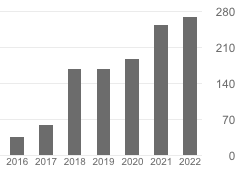
\includegraphics[height=30pt]{scholar-cit.png}

{\textsc{Full Publication list available \link{https://scholar.google.com/citations?user=ASf9Q04AAAAJ&hl=en}{\title{here}} }}

\begin{pubs}
	
	\confentryShort
	{1}
	{{\bf Ferdinando Fioretto} and Pascal Van Hentenryck}
	{Differential Privacy in Artificial Intelligence: From Theory to Practice}
	{Now Publisher, 2025}
	{https://www.barnesandnoble.com/w/differential-privacy-in-artificial-intelligence-ferdinando-fioretto/1146729617}

	\confentryShort
	{2} 
	{Vladimir Dvorkin, {\bf Ferdinando Fioretto}, Pascal Van Hentenryck, Pierre Pinson, Jalal Kazempour}
	{Privacy-Preserving Convex Optimization: When Differential Privacy Meets Stochastic Programming}
	{\venue{IEEE Conference on Decision and Control (CDC)}, 2025}
	{https://arxiv.org/abs/2209.14152}

	\confentryShort
	{3}
	{{Saswat Das}, {Jameson Sandler}, {\bf Ferdinando Fioretto}}
	{Disclosure Audits for LLM Agents}
	{\venue{NeurIPS} (under review), 2025}
	{https://www.arxiv.org/abs/2506.10171}

\confentryShort
	{4}
	{Prakhar Ganesh, \student{Cuong Tran}, Reza Shokri, {\bf Ferdinando Fioretto}}
	{The Data Minimization Principle in Machine Learning}
	{\procFAccT, 2025}
	{https://arxiv.org/abs/2405.19471}

\confentryShortAwd
	{5}
	{{Jacob K.~Christopher}, {Michael Cardei}, Brian R Bartoldson, Bhavya Kailkhura, {\bf Ferdinando Fioretto}}
	{Speculative Diffusion Decoding: Accelerating Language Generation through Diffusion}
	{\procNAACL, 2025}
	{https://arxiv.org/abs/2408.0563605246}
	{Oral}

\confentryShort
	{6}
	{{\bf Ferdinando Fioretto}, Diptangshu Sen, Juba Ziani}
	{Differentially Private Data Release on Graphs: Inefficiencies and Unfairness}
	{\procAISTATS, 2025}
	{https://arxiv.org/abs/2408.05246}

\confentryShortAwd
	{7}
	{{Joonhyuk Ko}, Juba Ziani, {Saswat Das}, Matt Williams, {\bf Ferdinando Fioretto}}
	{Fairness Issues and Mitigations in (Differentially Private) Socio-demographic Data Processes}
	{\procAAAI, 2025}
	{https://arxiv.org/abs/2408.08471}
	{Oral}

% \confentryShort
% 	{6}
% 	{Khang Tran, {\bf Ferdinando Fioretto}, Issa Khalil, My T.~Thai, NhatHai Phan}
% 	{FairDP: Certified Fairness with Differential Privacy}
% 	{In \venue{IEEE Secure and Trustworthy Machine Learning Conference (SaTML 2025)}, 2025}
% 	{https://arxiv.org/abs/2305.16474}

\confentryShort
	{8}
	{Sree Nelaturu, N.~Ravichandran, Cuong Tran, Sara Hooker, and {\bf Ferdinando Fioretto}}
	{On The Fairness Impacts of Hardware Selection in Machine Learning}	
	{\procICML, 2024}
	{https://arxiv.org/abs/2312.03886}

\confentryShort
	{9}
	{Saswat Das, Marco Romanelli, {\bf Ferdinando Fioretto}}
	{Disparate Impact on Group Accuracy of Linearization for Private Inference}
	{\procICML, 2024}
	{https://arxiv.org/abs/2402.03629}
	
% \confentryShort
% 	{9}
% 	{My H.~Dinh, James Kotary, {\bf Ferdinando Fioretto}}
% 	{End-to-End Learning for Fair Multiobjective Optimization Under Uncertainty}
% 	{\procUAI, 2024}
% 	{https://arxiv.org/abs/2402.07772}

\confentryShort
	{10}%{ArXiv}
	{Cuong Tran, Keyu Zhu, Pascal Van Hentenryck, {\bf Ferdinando Fioretto}}
	{Fairness Increases Adversarial Vulnerability}
	{\procIJCAI, 2024}
	{https://arxiv.org/abs/2211.11835}

\confentryShort
	{11}
	{My H.~Dinh, James Kotary, {\bf Ferdinando Fioretto}}
	{Learning Fair Ranking Policies via Differentiable Optimization of Ordered Weighted Averages}
	{\procFAccT, 2024}
	{https://arxiv.org/abs/2402.05252}

\confentryShort
	{12}
	{{\bf Ferdinando Fioretto}, Keyu Zhu, Pascal Van Hentenryck, Saswat Das, Christine Task}
	{Finding $\epsilon$ and $\delta$ of Traditional Disclosure Control Systems}
	{\procAAAI, 2024}
	{https://arxiv.org/abs/2301.12204}

\confentryShort
	{13}
	{{Cuong Tran} and {\bf Ferdinando Fioretto}}
	{Data Minimization at Inference Time}
	{\procNeurIPS, 2023}
	{https://arxiv.org/abs/2305.17593}

% \confentryShort
%  {13} %{IJCAI}
% 	{{James Kotary}, {Vincenzo Di Vito}, {\bf Ferdinando Fioretto}, Pascal Van Hentenryck}
% 	{SF-PATE: Scalable, Fair, and Private Aggregation of Teacher Ensembles}
%   {\procIJCAI, 2023}
% 	{https://arxiv.org/abs/2204.05157}

\confentryShort
  {14} %{IJCAI}
	{{Cuong Tran}, {\bf Ferdinando Fioretto}}
	{On the Fairness Impacts of Private Ensembles Models}
    {\procIJCAI, 2023}
	{http://arxiv.org/abs/2109.08630}

\confentryShortAwd
	{15} %{NeurIPS}
	{{Cuong Tran}, {\bf Ferdinando Fioretto}, Jung-Eun Kim, {Rakshit Naidu}}
	{Pruning has a disparate impact on model accuracy}
	{\procNeurIPS, 2022}
	{http://arxiv.org/abs/2205.13574}
	{Spotlight}

	\confentryShort
	{16} %{IJCAI}
	{Keyu Zhu, {\bf Ferdinando Fioretto}, Pascal Van Hentenryck}
	{Post-processing of Differentially Private Data: A Fairness Perspective}
	{\procIJCAI, 2022}
	{http://arxiv.org/abs/2202.09425}	

	\confentryShort
	{17} %{IJCAI}
	{{\bf Ferdinando Fioretto}, {Cuong Tran}, Keyu Zhu, Pascal Van Hentenryck}
	{Differential Privacy and Fairness in Decisions and Learning Tasks: A Survey}
	{\procIJCAI, 2022}
	{http://arxiv.org/abs/2202.08187}	

	% \confentryShort
	% {22} %{WWW}
	% {{James Kotary}, {\bf Ferdinando Fioretto}, Pascal Van Hentenryck, Ziwei Zhu}
	% {End-to-end Learning for Fair Ranking Systems}
	% {\procWWW, 2022}
	% {http://arxiv.org/abs/2111.10723}	

	\confentryShort 
	{18} %{NeurIPS}
	{{Cuong Tran}, {My H.~Dinh}, {\bf Ferdinando Fioretto}}
	{Differentially Private Deep Learning under the Fairness Lens}
	{\procNeurIPS, 2021}
	{https://arxiv.org/pdf/2106.02674.pdf}

	\confentryShortAwd 
	{19} %{IJCAI}
	{{Cuong Tran}, {\bf Ferdinando Fioretto}, Pascal Van Hentenryck, {Zhiyan Yao}}
	{Decision Making with Differential Privacy under the Fairness Lens}
	{\procIJCAI, 560--566, 2021}
	{https://www.ijcai.org/proceedings/2021/78}
	{2022 Caspar Bowden PET Award}

	\confentryShort 
	{20} %{AAAI}
	{Keyu Zhu, Pascal Van Hentenryck, {\bf Ferdinando Fioretto}}
	{Bias and Variance of Post-processing in Differential Privacy}
	{\procAAAI, 11177--11184, 2021}
	{https://ojs.aaai.org/index.php/AAAI/article/view/17333}

	% \confentryShort
	% {20} %{IJCAI}
	% {{\bf Ferdinando Fioretto}, Lesia Mitridati, Pascal Van Hentenryck}
	% {Differential Privacy Stackebelg Games}
	% {\procIJCAI, 3480--3486, 2020}
	% {https://www.ijcai.org/proceedings/2020/0481.pdf}

\end{pubs}

% \sectionTitle{Mentorship and Impact, in Numbers}{}%{\faBook}
% {\bf Mentorship}: Currently mentoring 8 PhD students and 3 undergraduate students. \hspace{20pt}
% Previously mentored 20+ undergraduate students, 5 MS students, and 5 PhD students.\\
% {\bf Invited Talks and Media Engagements}: Delivered over 60 talks and media interviews.\\
% {\bf Research Funds}: External: \$2.85M (\$2.39M as PI) \hspace{4pt}|\hspace{4pt} Internal: \$81K

\vspace{6pt}
\sectionTitle{Selected Synergistic Activities}{}%{\faBook}
\vspace{6pt}
  \begin{itemize}
  	\item {\bf Editorial Board Member:}\\
  	Artificial Intelligence Journal \hfill{2024 -- current}\\
  	Journal of Artificial Intelligence Research \hfill{2024 -- current}
		%Associate Editor for IISE Transactions Special issue on Federated Learning  \hfill{2024}

    \item {\bf Conference co-chair and Organizing Committee}:  \\
		{\bf Tutorial Chair:} The ACM International Conference on AI in Finance (ICAIF) \hfill{2025}\\
    %{\bf Track Chair:} International Joint Conference on Artificial Intelligence (IJCAI) \hfill{2023}\\
		% {\bf Scholarship Chair:} International Conference on Autonomous Agents and Multiagent Systems (AAMAS) \hfill{2023}\\
		{\bf Tutorial Chair}:  International Conference on Autonomous Agents and Multiagent Systems (AAMAS) \hfill{2022}\\
    {\bf Conference Chair:} International Conference on Principles and Practice of Constraint Programming (CP)  \hfill{2022}
		
    \item {\bf Workshop co-organizer}: \\
    {Workshop on Privacy Preserving Artificial Intelligence, (at AAAI)}   \hfill{2020 -- 2026}\\
    {Workshop on Optimization and Learning in Multi-Agent Systems, at AAMAS} \hfill{2018 -- 2022}\\
    {Algorithmic Fairness through the Lens of Causality and Privacy, (at NeurIPS)} \hfill{2022 -- 2025}
    %{Workshop on Machine Learning for Operational Research, (at AAAI)}   \hfill{2022, 2024}
    
    \item {\bf (Senior) Area Chair}: \\
    AAAI Conference on Artificial Intelligence (AAAI) \hfill {2020 -- 2026}\\
    International Joint Conference on Artificial Intelligence (IJCAI) \hfill {2021 -- 2025}\\
    International Conference on Machine Learning (ICML) \hfill {2025}\\
    ACM Conference on Fairness, Accountability, and Transparency (FAccT) \hfill {2023 -- 2025}\\
    %European Conference on Machine Learning (ECML) \hfill{2023 -- 2024}\\
  	%European Conference on Artificial Intelligence (ECAI) \hfill {2023 -- 2024}\\
  	Conference on Neural Information Processing Systems (NeurIPS) \hfill {2023 -- 2025} \\
    International Conference on Autonomous Agents and Multiagent Systems (AAMAS) \hfill{2024}
  \end{itemize}


\end{document}